\documentclass[tikz,border=10pt]{standalone}
\begin{document}
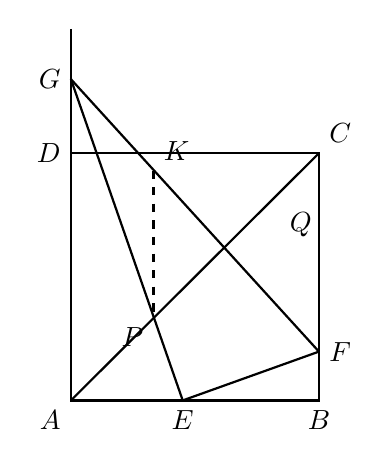
\begin{tikzpicture}[thick]
  % Points
  \coordinate (A) at (0,0);
  \coordinate (B) at (3.15,0);
  \coordinate (C) at (3.15,3.14);
  \coordinate (D) at (0,3.14);
  \coordinate (E) at (1.42,0);
  \coordinate (F) at (3.15,0.62);
  \coordinate (G) at (0,4.08);
  \coordinate (K) at (1.05,2.92);
  \coordinate (P) at (1.05,1.06);
  \coordinate (Q) at (2.65,1.95);

  % Square and extended vertical line
  \draw (0,4.72) -- (A) -- (B) -- (C) -- (D);

  % Diagonal AC
  \draw (A) -- (C);

  % Lines through G
  \draw (G) -- (E);
  \draw (G) -- (F);

  % Segment EF
  \draw (E) -- (F);

  % Dashed segment from K down to P
  \draw[dashed] (K) -- (P);

  % Labels
  \node[anchor=north east] at (A) {$A$};
  \node[anchor=north] at (B) {$B$};
  \node[anchor=south west] at (C) {$C$};
  \node[anchor=east] at (D) {$D$};
  \node[anchor=north] at (E) {$E$};
  \node[anchor=west] at (F) {$F$};
  \node[anchor=east] at (G) {$G$};
  \node[anchor=south west] at (K) {$K$};
  \node[anchor=north east] at (P) {$P$};
  \node[anchor=south west] at (Q) {$Q$};
\end{tikzpicture}
\end{document}
